\chapter{Detection of Gravitational-Wave Signals from Binary Neutron Star Mergers using Machine Learning}\label{ch:bns}
\chaptermark{Binary Neutron Star Search using Machine Learning}
This chapter briefly summarizes the work done in \cite{Schafer:2020kor}, which in turn is based on my master thesis \cite{Schaefer:2019:MSC}. It highlights the improvements of \cite{Schafer:2020kor} over \cite{Schaefer:2019:MSC}. It is discussed in this thesis, as the detection of long duration \acrshort{gw} signals from \acrshort{bns} mergers is a major challenge in machine learning based search algorithms.

\section{Introduction}
Long duration \acrshort{bns} signals are computationally expensive to search for using matched filtering. This is an effect of the required high density of templates in the bank at low masses. On the other hand, detecting \acrshort{bns} signals with as low a latency as possible is important to maximize \acrshort{em} observation time of potential counterparts.

One possible approach to try to reduce computational demands of the search is to employ advanced \acrshort{ml} methods, that shift the computational cost to the training phase. To prove they are capable of rapid and accurate detection, these algorithms must be evaluated at \acrshort{far}s that are at a level comparable to online production search pipelines~\cite{Nitz:2018rgo}. In this study, we develop a deep learning search algorithm for \acrshort{bns} signals. We compare it to the PyCBC Live pipeline which has been used in the online analysis of \acrshort{o2} and \acrshort{o3}. We also compare our algorithm to another deep learning based search that targets \acrshort{bns} mergers.

The core problem of developing deep learning based \acrshort{bns} search algorithms is the duration the signal spends in the sensitive bands of the detectors. This long duration in combination with a merger at high frequencies results in a large number of samples that have to be processed. When the size of the input to a \acrshort{nn} grows, so must typically the size of the network~\cite{Goodfellow:2016:DNN}. This makes training unfeasible due to excessive hardware requirements. Our solution to this problem is to use the knowledge of the frequency evolution of \acrshort{bns} signals to re-sample different parts of the data at different rates.

\section{Methods}
To reduce the number of samples in the input to the \acrshort{nn} we sample the data at different rates. During the early inspiral the frequency is low and evolves slowly. As a consequence, a low sample rate is sufficient to resolve the signal for a long duration. Only close to the merger are high frequencies involved and a high sample rate is necessary. Informed by this signal evolution, we re-sample the first \SI{16}{\second} of the input data at a rate of \SI{128}{\hertz}. The next \SI{8}{\second} are sampled at a rate of \SI{256}{\hertz}. We continue doubling the sample rate and halving the duration of data we sample until the final second of our \SI{32}{\second} input data. The final second is split into two \SI{0.5}{\second} parts, each sampled at \SI{4096}{\hertz}. This procedure reduces the number of samples by a factor of 9, while the \acrshort{snr} that is lost due to the early truncation at low frequencies is only $\approx 2\%$. In \cite{Schaefer:2019:MSC} we had re-sampled \SI{64}{\second} by starting with a sample rate of \SI{64}{\hertz} for the first \SI{32}{\second} part. However, we found that for some signals the maximum frequency in that time period exceeded the limit of \SI{32}{\hertz} set by the sampling rate. See \autoref{fig:bns_resample} for a visualization of the re-sampling process. 
\begin{figure}
	\centering
	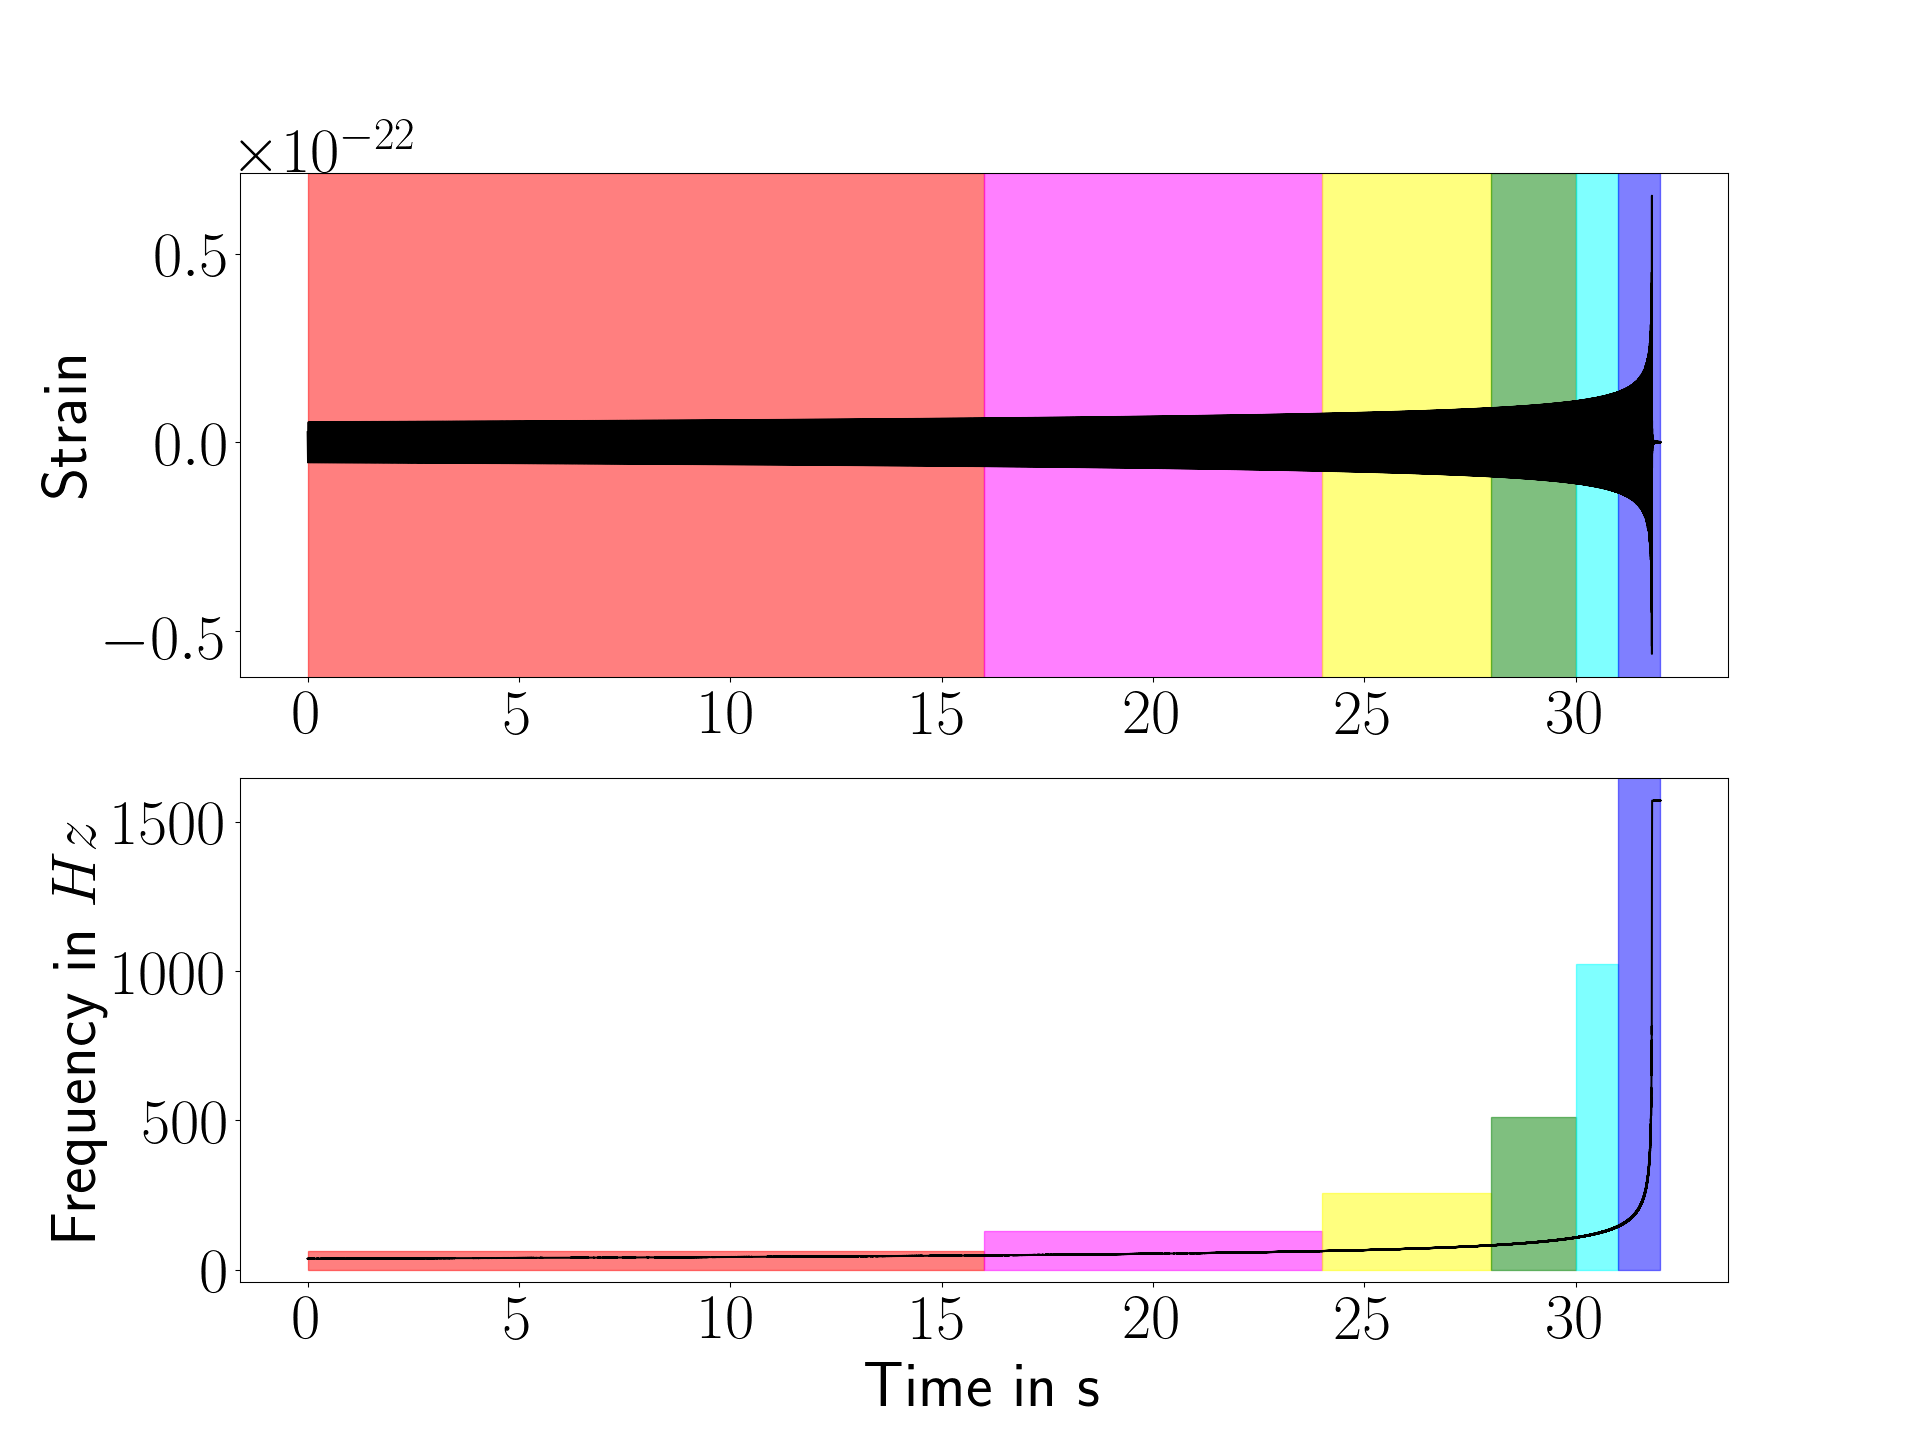
\includegraphics[width=0.8\textwidth]{chapters/bnsnet/images/resample_idea.png}
	\caption[Multi-rate sampling]{The top panel shows the strain evolution of an example \acrshort{gw} from a \acrshort{bns} merger in black. The bottom panel shows the corresponding frequency evolution in black. The colored boxes represent parts of the signal which we sample at different rates. The height of these boxes in the bottom panel represents the Nyquist-frequency of the sample rate which is used for each part. To fully resolve the signal, the black curve must stay inside the colored boxes of the bottom panel at all times. Figure and caption were taken from \cite{Schafer:2020kor}.}\label{fig:bns_resample}
\end{figure}

The architecture used in \cite{Schafer:2020kor} is highly adjusted to the multi-rate sampled data. Each of the $7$ different parts of the input data is processed by a different input to the network. After each sample rate has been processed individually, pairs of two are combined and processed further. This structure cascades down until only a single branch remains. This single branch is processed by a few more layers to produce two outputs: An estimate of the optimal \acrshort{snr} contained in the input and a p-score that is a value between $0$ and $1$ signifying the confidence of the network that a signal is present in the input. A high-level overview of the architecture is given in \autoref{fig:bns_architecture}. For more details see \cite{Schafer:2020kor, Schaefer:2019:MSC}. The architecture is the same as the one presented in \cite{Schaefer:2019:MSC}, adjusted to the reduced number of multi-rate sampled parts.
\begin{sidewaysfigure*}
	\centering
	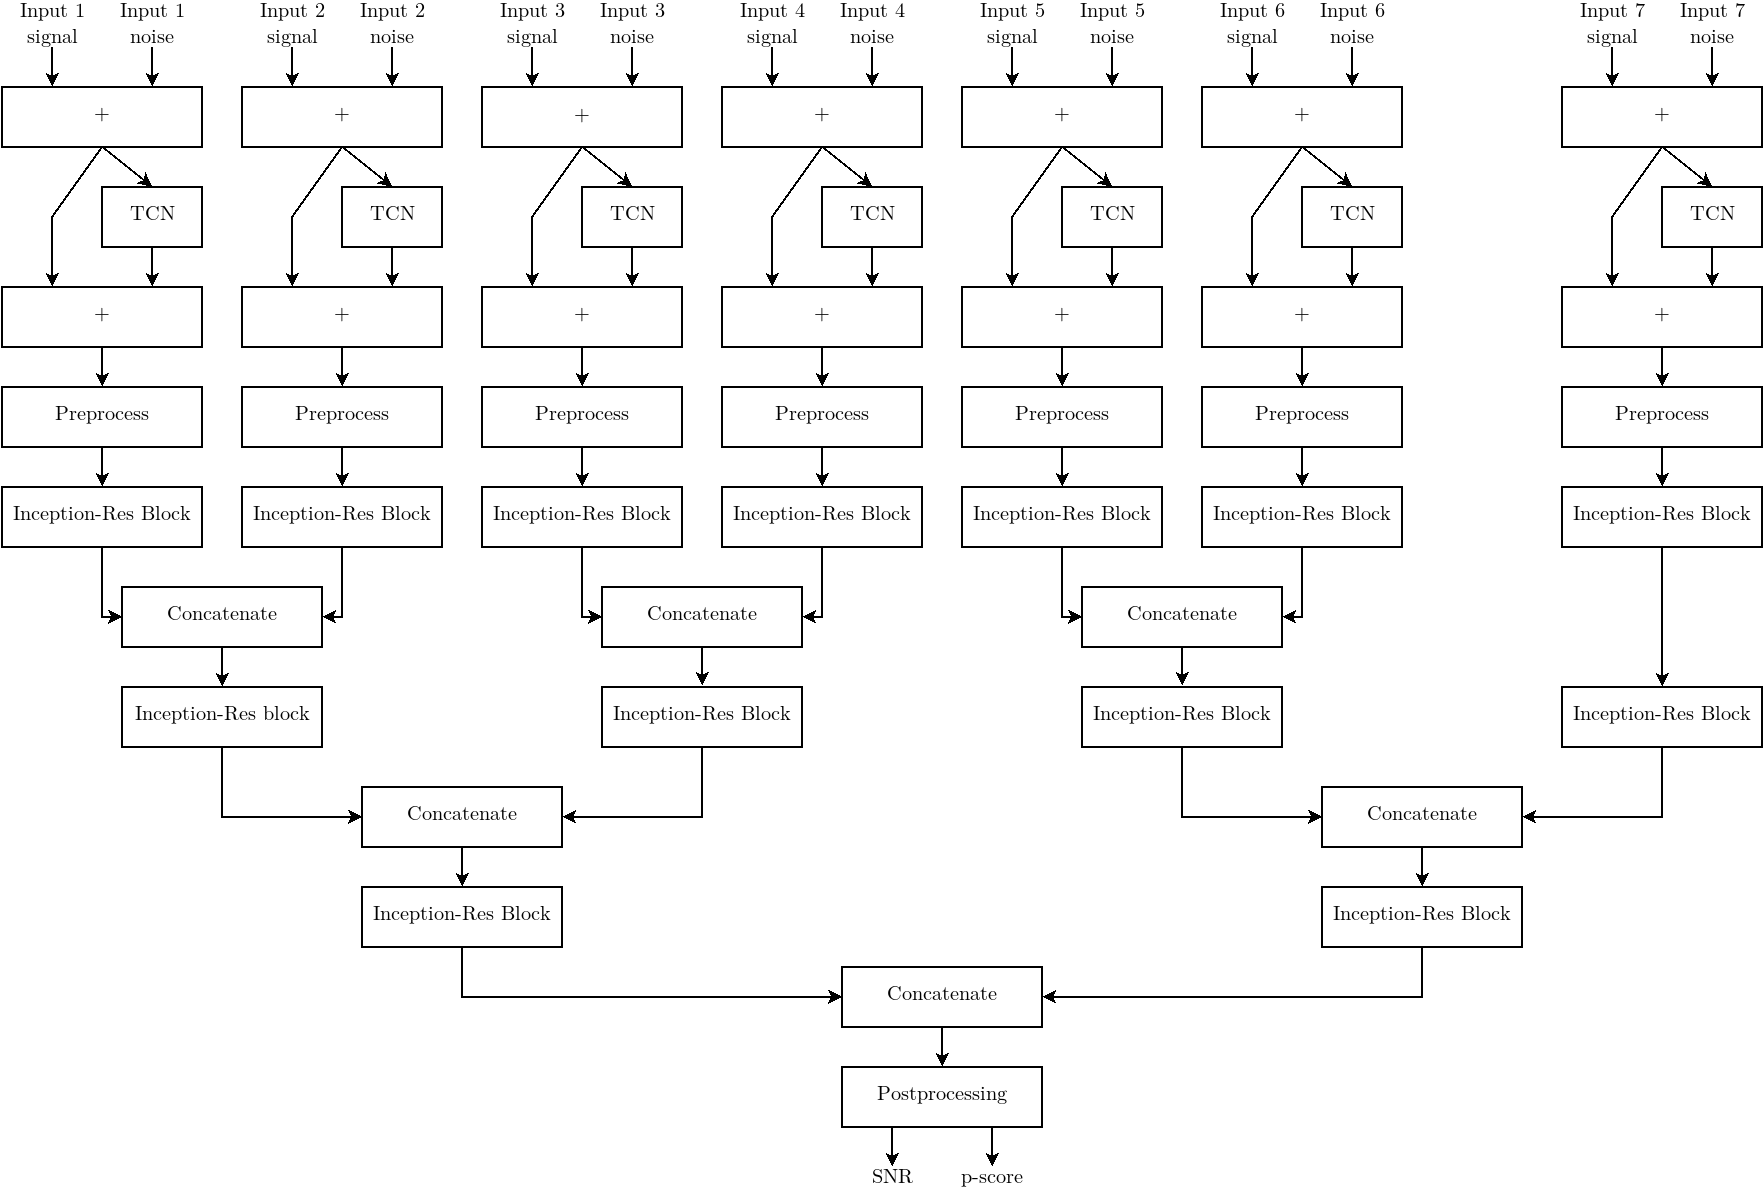
\includegraphics[width=0.9\textwidth]{chapters/bnsnet/images/architecture.png}
	\caption[Architecture]{A high level overview of the architecture presented in \cite{Schafer:2020kor}. Details on every block can be found in \cite{Schaefer:2019:MSC}. The network takes signal and noise inputs $1$ to $7$, where each number corresponds to a different part of the re-sampled raw data. It outputs an estimate of the \acrshort{snr} contained in the input and a p-score, which rates how likely the data is to contain a \acrshort{bns} signal. Figure and caption were taken from \cite{Schafer:2020kor}.}\label{fig:bns_architecture}
\end{sidewaysfigure*}

Training and validation data were created by the same process. Noise is simulated from the advanced \acrshort{ligo} design sensitivity curve in its zero detuned high-power configuration~\cite{lalsuite}. Signals are generated using the TaylorF2 waveform approximant~\cite{Droz:1999qx, Blanchet:2006aaa, Faye:2012we}, with all parameters except for the distance $r$ drawn from \autoref{tab:bns_parameter_distribution}. The distance is set indirectly by fixing the optimal \acrshort{snr} to a value uniformly drawn between $8$ and $15$. For each sample in the training set, we generate \SI{96}{\second} of data, whiten it by the \acrshort{psd} model, and crop the resulting data to \SI{32}{\second}. The exact position of the merger time in the final data is varied by \SI[parse-numbers=false]{\pm 0.25}{\second}. We create noise for the \acrshort{ligo}-Hanford and \acrshort{ligo}-Livingston detectors and inject the projected waveforms into both. The test set consists of $\approx 101$ days of continuous data split into multiple files. Injections are generated using the same waveform model and the distributions of \autoref{tab:bns_parameter_distribution}. They are spaced by \SIrange{180}{220}{\second}. Our work in \cite{Schafer:2020kor} corrects an error from \cite{Schaefer:2019:MSC} where the \acrshort{psd} was sampled too coarsely. This reduced the \acrshort{snr} of the signals below the expected value.
\begin{table}
\centering
\begin{tabular}{ll}
	\hline\hline
    parameter & uniform distribution\\
    \hline\\
    component masses & \SI[parse-numbers=false]{m_1, m_2\in\left(1.2,1.6\right)}{M_\odot}\\
    spins & 0\\
    coalescence phase & $\Phi_0\in\left(0, 2\pi\right)$\\
    polarization & $\Psi\in\left(0, 2\pi\right)$\\
    inclination & $\cos{\iota}\in\left(-1, 1\right)$\\
    declination & $\sin{\theta}\in\left(-1, 1\right)$\\
    right ascension & $\varphi\in\left(-\pi, \pi\right)$\\
    distance & \SI[parse-numbers=false]{r^2\in\left(0^2, 400^2\right)}{{\mega\parsec}^2}\\
    \hline\hline
\end{tabular}
\caption[Parameter distributions]{The astrophysically motivated distribution of parameters used to generate injections. These are used to estimate the \acrshort{far} and sensitivity of the search algorithm specified in \cite{Schafer:2020kor}. Table and caption were taken from \cite{Schafer:2020kor}.}\label{tab:bns_parameter_distribution}
\end{table}

To apply the network to data of duration longer than the input, i.e. \SI{32}{\second}, a sliding window is used. Each window is whitened and re-sampled as described above. The window uses a step size of \SI{0.25}{\second}, matching the variation of the merger time in the training data. The outputs of the network are time series of \acrshort{snr} estimates and p-scores. We apply thresholds of \acrshort{snr} $4$ and p-score $0.1$ and cluster points exceeding the threshold if they are within \SI{1}{\second} of each other. Afterward, we compare the time of the maximum value of each cluster with the injections to determine true and false positive detections. We accept something as true positive, if it is within \SI{3}{\second} of an injection.

\section{Results}
The sensitivity of our proposed algorithm is summarized in \autoref{fig:bns_sensitivity}. Our testing procedure allows us to calculate sensitivities down to a \acrshort{far} of $0.3$ per month. We find that the \acrshort{snr} output collapses to zero sensitivity below a \acrshort{far} of $0.6$ per month, while the p-score collapses already at a \acrshort{far} of $12$ per month. This is an improvement over \cite{Schaefer:2019:MSC}, which was incapable of resolving \acrshort{far}s below $30$ per month. The algorithm shows non negligible sensitivity down to a \acrshort{far} of $10$ per month in the \acrshort{snr} output and $20$ per month in the p-score output, where it reaches a sensitive distance of \SI[parse-numbers=false]{\approx 130}{\mega\parsec}. We also find that at low \acrshort{far}s the \acrshort{snr} output is more sensitive than the p-score output, which stands in contrast to our previous findings in \cite{Schaefer:2019:MSC}.
\begin{figure}
	\centering
	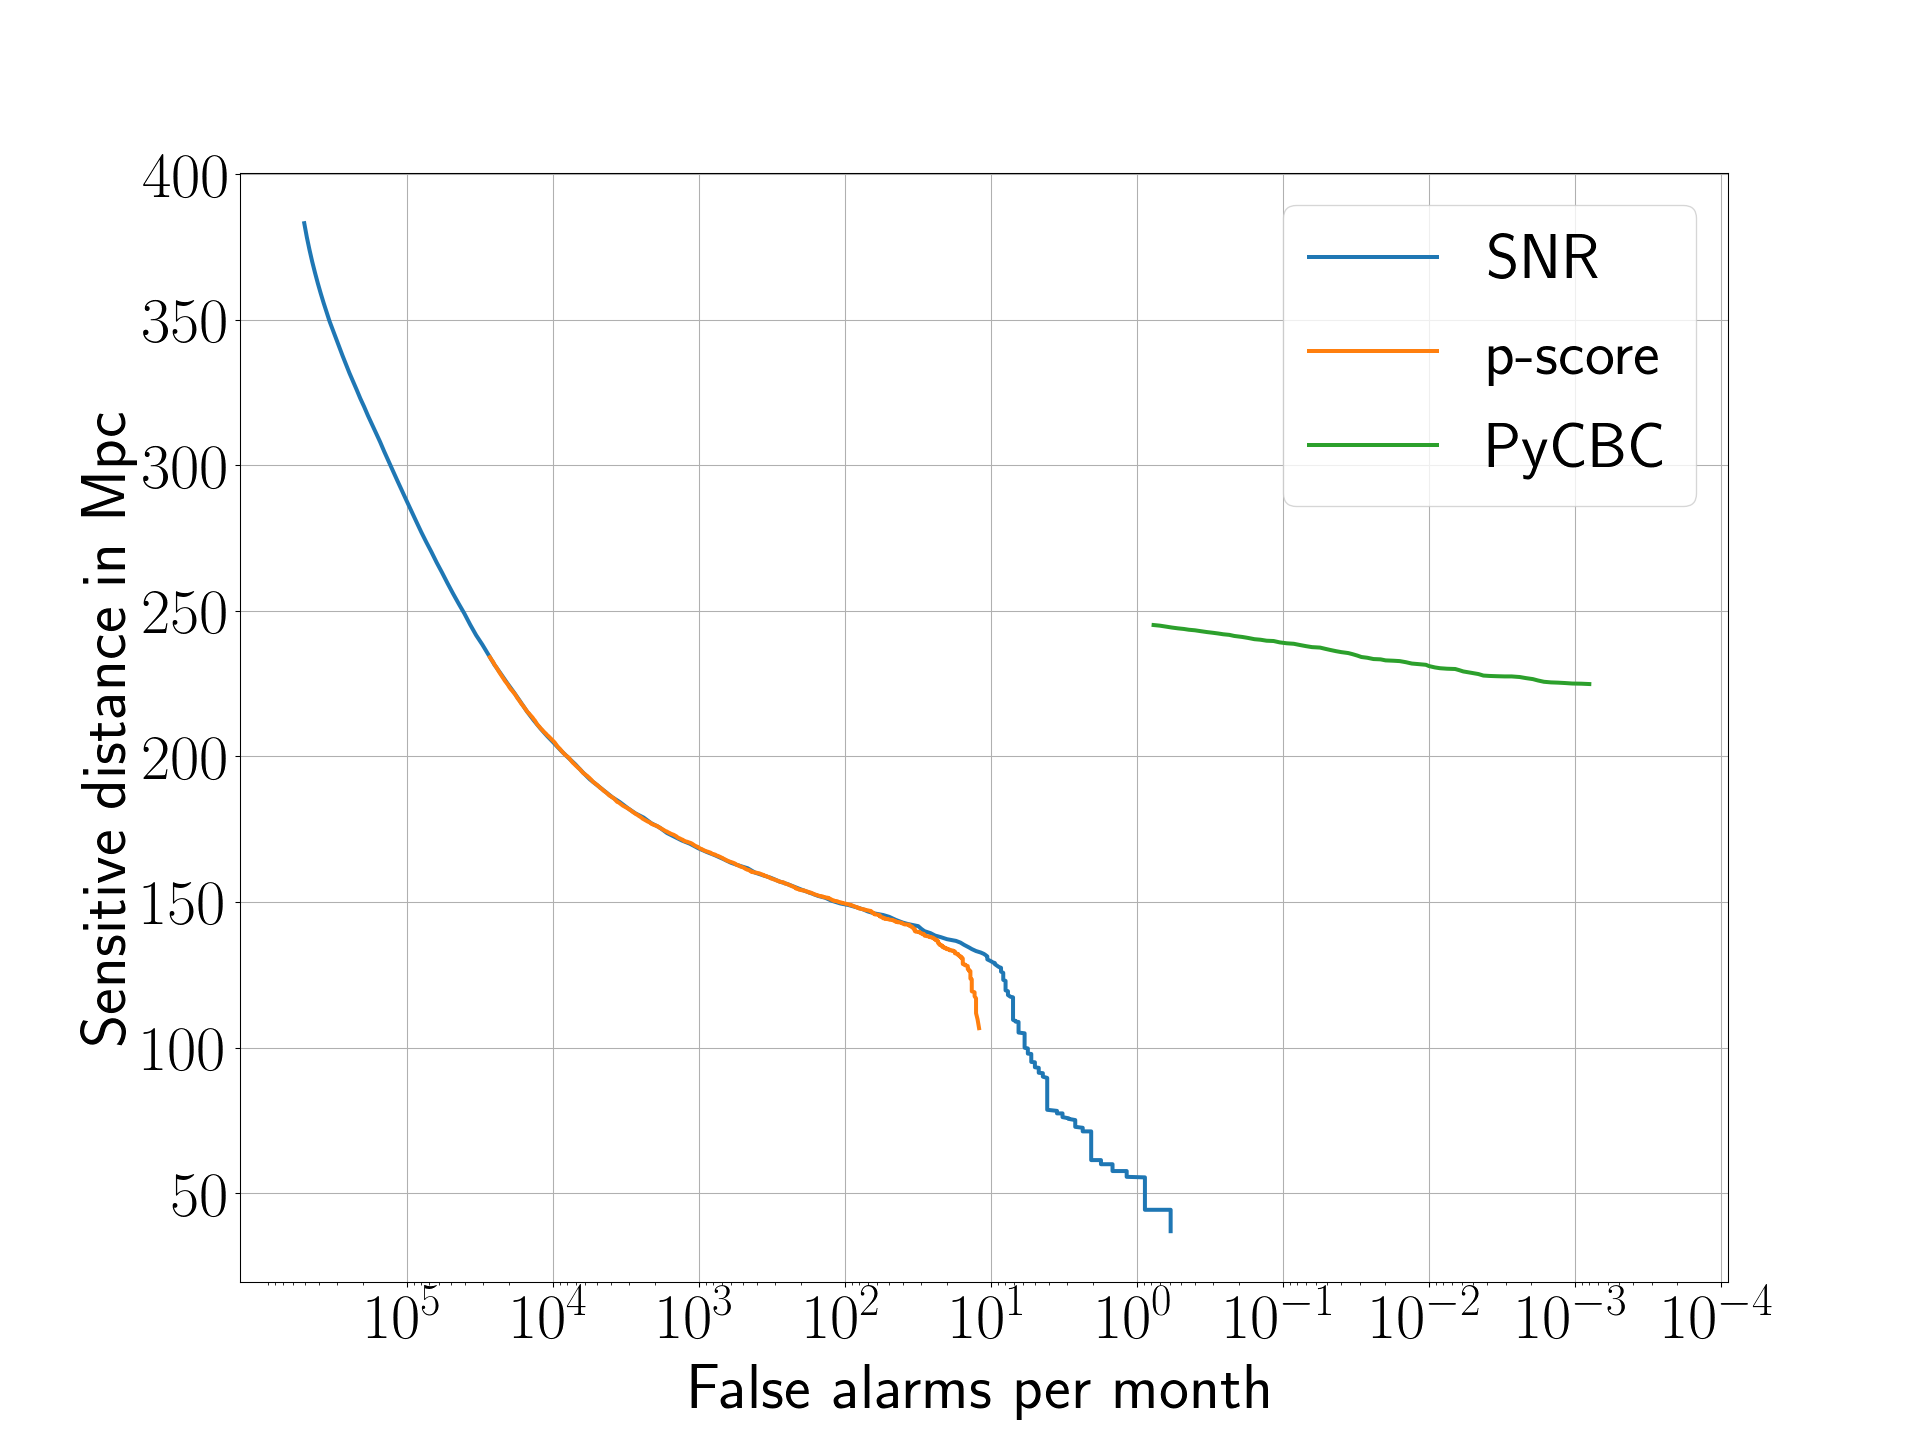
\includegraphics[width=0.8\textwidth]{chapters/bnsnet/images/SensitivitySNR}
	\caption[Sensitivity]{The sensitive distance as a function of the \acrshort{far}. The blue curve shows the sensitive distance when the \acrshort{snr} is used to classify events. The yellow curve shows the sensitive distance when the p-score is used. The green curve is generated from the data found in \cite{Nitz:2017svb} by counting all signals at a higher injection \acrshort{snr} than the corresponding \acrshort{far}. We are able to resolve a small overlap-region between the two different searches but find that the sensitivity of our search drops close to zero for \acrshort{far}s below 10 per month. At high \acrshort{far}s both outputs of our network perform equally well, for low \acrshort{far}s the \acrshort{snr} shows superior performance. Figure and caption were taken from \cite{Schafer:2020kor}.}\label{fig:bns_sensitivity}
\end{figure}

We compare our analysis to PyCBC Live~\cite{Nitz:2018rgo}. To estimate the sensitivity of PyCBC Live, we use Figure 1 from \cite{Nitz:2017svb} to obtain a ranking statistic $\mathcal{R}$ as a function of \acrshort{far}. We then assume that all injections with optimal network \acrshort{snr} $> \mathcal{R}$ are found by PyCBC Live. The green curve in \autoref{fig:bns_sensitivity} shows the resulting sensitivity curve. We find that PyCBC Live achieves about twice the sensitive distance measured for our algorithm at a \acrshort{far} lower by about one order of magnitude. We also measure the latency introduced by our algorithm to compare it to the latency of PyCBC live. Ignoring pre-processing, our algorithm is capable of producing alerts in real time and introduces an average latency of \SI{10.2}{\second}. Restricting PyCBC Live to the parameter region of \autoref{tab:bns_parameter_distribution} results in a template bank containing $1960$ templates per detector, which can be used to filter the data for both detectors on a single \acrshort{cpu} core in real time. This analysis also introduces a latency of $\mathcal{O}(10)$ seconds, making it at least as computationally efficient as our deep learning alternative.

We also compare our search algorithms to another deep learning based \acrshort{bns} signal detection pipeline published as \cite{Krastev:2019koe}. The original pre-print \cite{Krastev:2019aaa} was revised before publication as \cite{Krastev:2019koe} shortly before we published our study. For this reason we compare our approach to both versions. The pre-print study~\cite{Krastev:2019aaa} gave signal strength in terms a peak signal-to-noise ratio (\acrshort{psnr}), which we estimate to be related to optimal \acrshort{snr} by $\text{\acrshort{snr}}=41.2\text{\acrshort{psnr}}$. Both the pre-print as well as the published version operate only on data from a single detector, whereas our algorithm uses data from two detectors. For this reason, we also scale the \acrshort{snr} from \cite{Krastev:2019aaa} and \cite{Krastev:2019koe} by a factor of $\sqrt{2}$ to estimate the network \acrshort{snr}. The comparison in terms of true positive rate can be found in \autoref{fig:bns_tpr} at different \acrshort{far}s. We find that our approach is about $4$ times as sensitive as the one presented in \cite{Krastev:2019koe} in the \acrshort{snr} region our network was trained on, which is marked by the gray area in the plot. However, our algorithm falls off rapidly for loud signals and only saturates at a sensitivity of $100\%$ for \acrshort{snr}s $>46.65$.
\begin{figure}
	\centering
	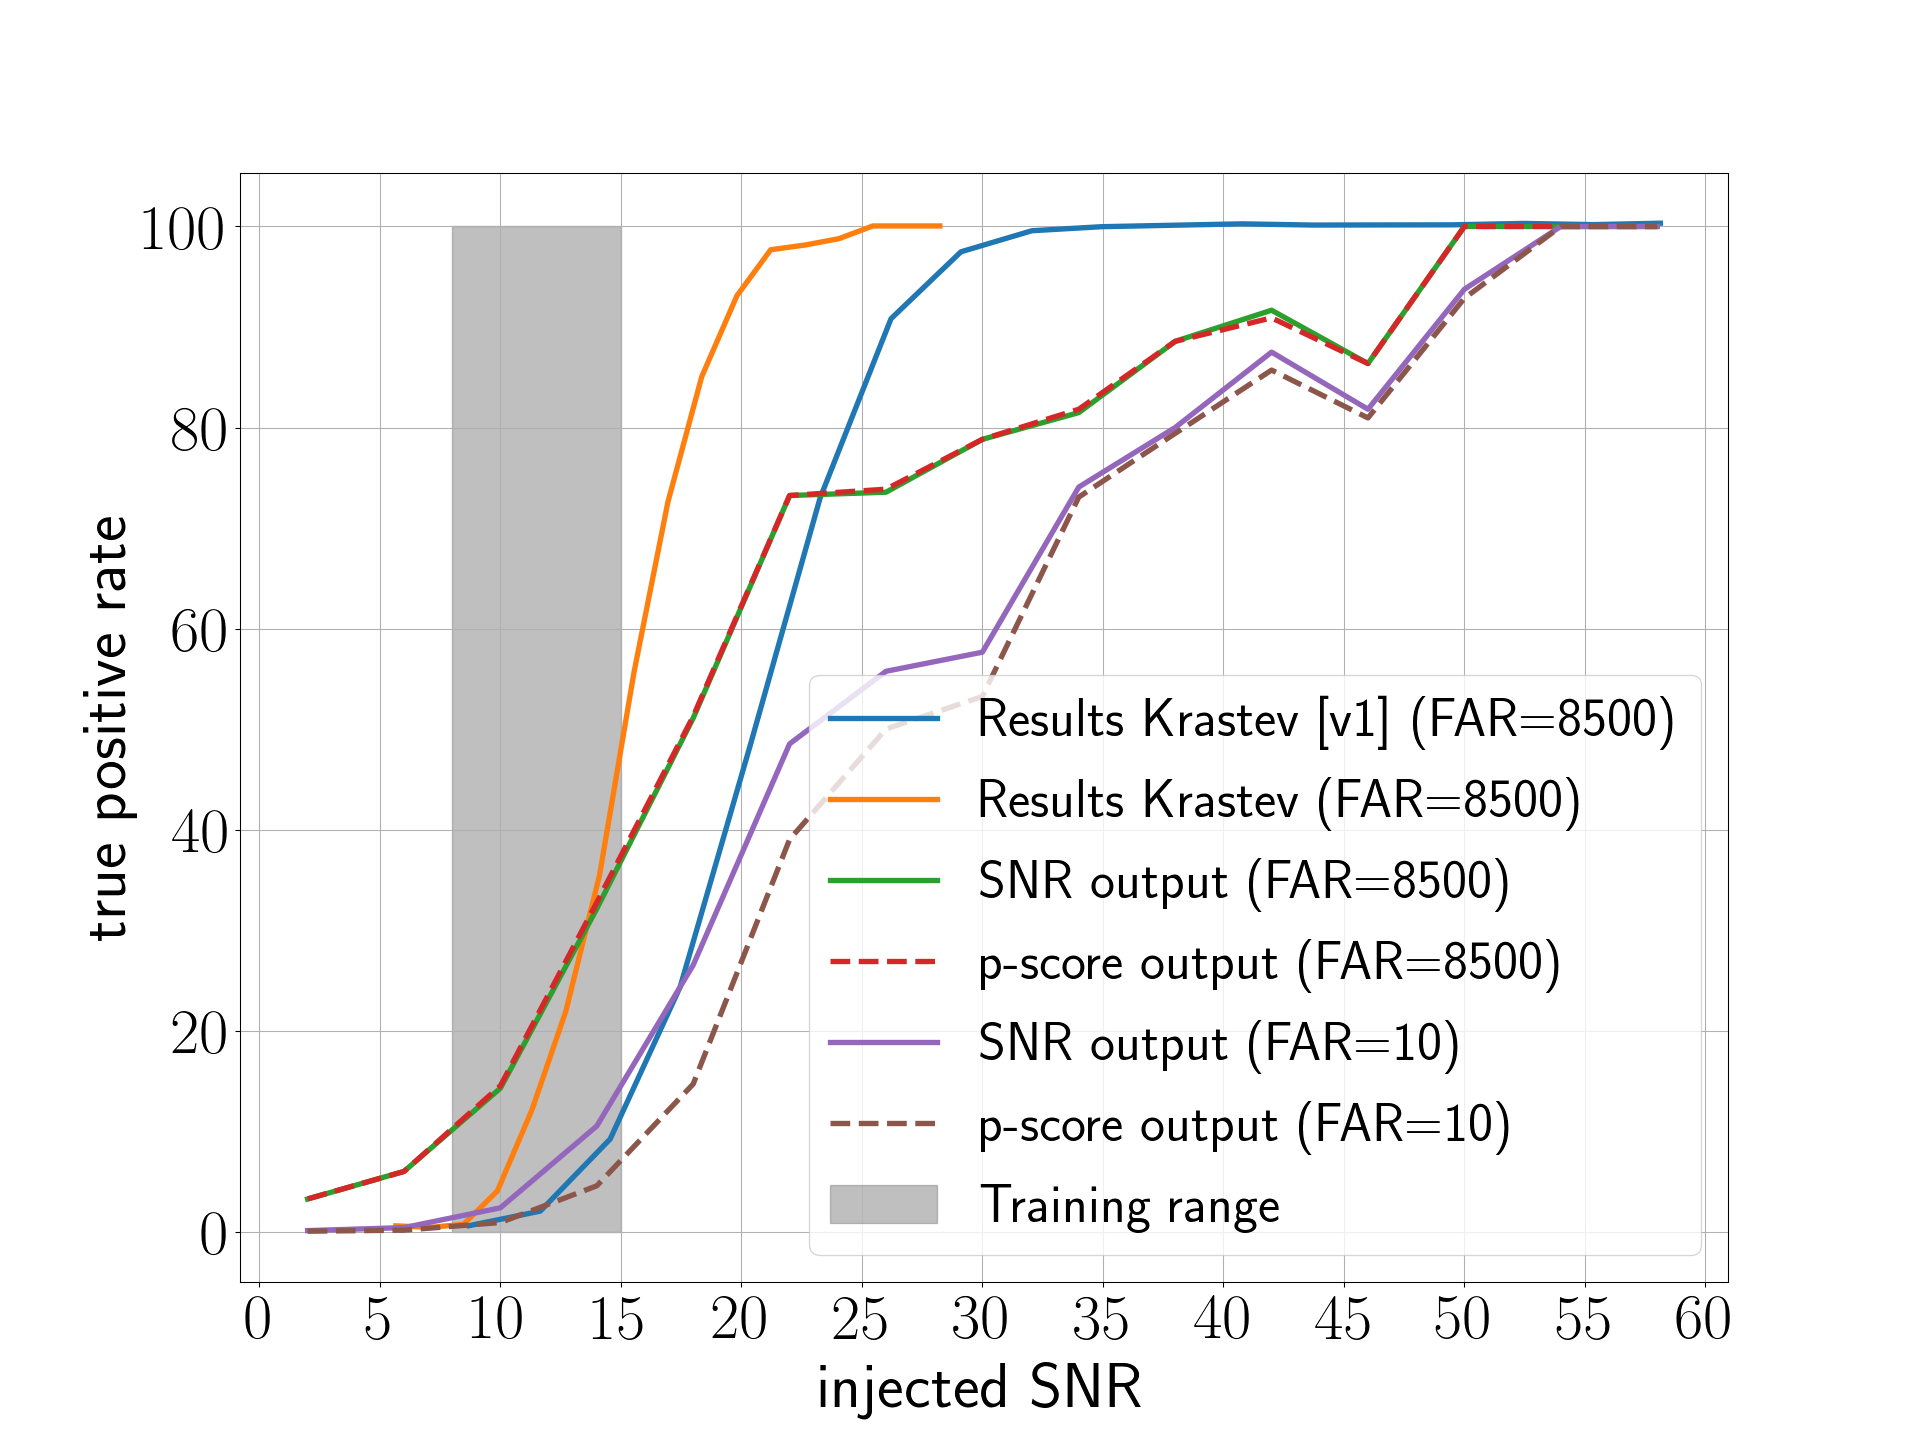
\includegraphics[width=0.8\textwidth]{chapters/bnsnet/images/compare_krastev_v2}
	\caption[True positive rate]{To compare our search to the work of \cite{Krastev:2019koe} we plot their true positive rate at a fixed \acrshort{far} of $8500$ per month in yellow and our true positive rate at the same \acrshort{far} in green and red. On the x-axis we track the injected optimal network \acrshort{snr}. The blue curve shows the data from \cite{Krastev:2019aaa}, where the results were given in terms of pSNR. We use the conversion $\text{\acrshort{snr}} = 41.2\cdot\sqrt{2}\cdot\text{pSNR}$. To obtain these curves we bin the injected signals by their optimal injection \acrshort{snr} and a bin size of 4. For high \acrshort{snr}s some bins are empty. Empty bins are interpolated linearly from the remaining data. The area marked gray highlights the region covered by the training set. We find that our search performs better for low \acrshort{snr}s but is less sensitive for strong signals. We also show the true positive rate of our search at a \acrshort{far} of 10 in purple and brown. Within the training range we find that our search closely matches the true positive rate of \cite{Krastev:2019aaa} at a higher \acrshort{far}. Figure and caption were taken from \cite{Schafer:2020kor}.}\label{fig:bns_tpr}
\end{figure}

\section{Conclusions}
We introduced a novel procedure of making long duration time domain data accessible to \acrshort{nn}s, by sampling the data at multiple rates. This multi-rate sampling was used to train and evaluate a deep learning based search algorithm for \acrshort{gw}s from \acrshort{bns} mergers. We compared it to the state-of-the-art matched filter based low-latency search pipeline PyCBC Live and found that it is neither computationally more efficient nor as sensitive. This shows that more work is required to build competitive deep learning search algorithms for complex signals.

We also compare our analysis to another deep learning \acrshort{bns} search algorithm. Our algorithm was approximately four times as sensitive to signals with \acrshort{snr} $\leq 15$ but could not generalize well to louder signals.

Finally, we proposed an evaluation scheme that produces results that are comparable to existing pipelines and is normalized to the injected population of \acrshort{gw} sources. We used this scheme to test our algorithm down to a \acrshort{far} of $0.3$ per month. This analysis showed that the sensitivity of our deep learning based algorithm drops to zero for \acrshort{far}s that are low compared to \acrshort{far}s at which deep learning algorithms are usually tested. Following \cite{Gebhard:2019ldz}, we argued that using \acrshort{fap}s, which are derived on discrete samples does not translate well to performance measures based on the more physically relevant \acrshort{far}s, as clustering effects are disregarded for \acrshort{fap}s.
